\documentclass[../Article_Sensitivity_Analsysis.tex]{subfiles}
\graphicspath{{\subfix{../Figures/}}}
\begin{document}
	
	\label{CH: Results}
	
	This work investigates the influence of inlet temperature, pressure, and mass flow rate on the state space and the extraction yield. The process model and parameters have been discussed in {\color{red}article 1}. The process model was calibrated on the set of experiments obtained at different operating conditions, $30 - 40^\circ C$, $100 - 200$ bar, and $3.33-6.67 \times 10^{-5}$ kg/s. The sensitivity analysis has been performed assuming that the system operates at $35^\circ C$, 150 bar and 5 $\times 10^{-5}$ kg/s.
	
	\subsection{Flow rate}
	
	The increase in the mass-flow rate affects the system simultaneously along the spatial direction by increasing the velocity but without affecting the thermodynamic state of the fluid. As a result, Figure \ref{fig:Sensitivty_F_P} shows no change in pressure during the simulation.
	
	\begin{figure}[h!]
		\centering
		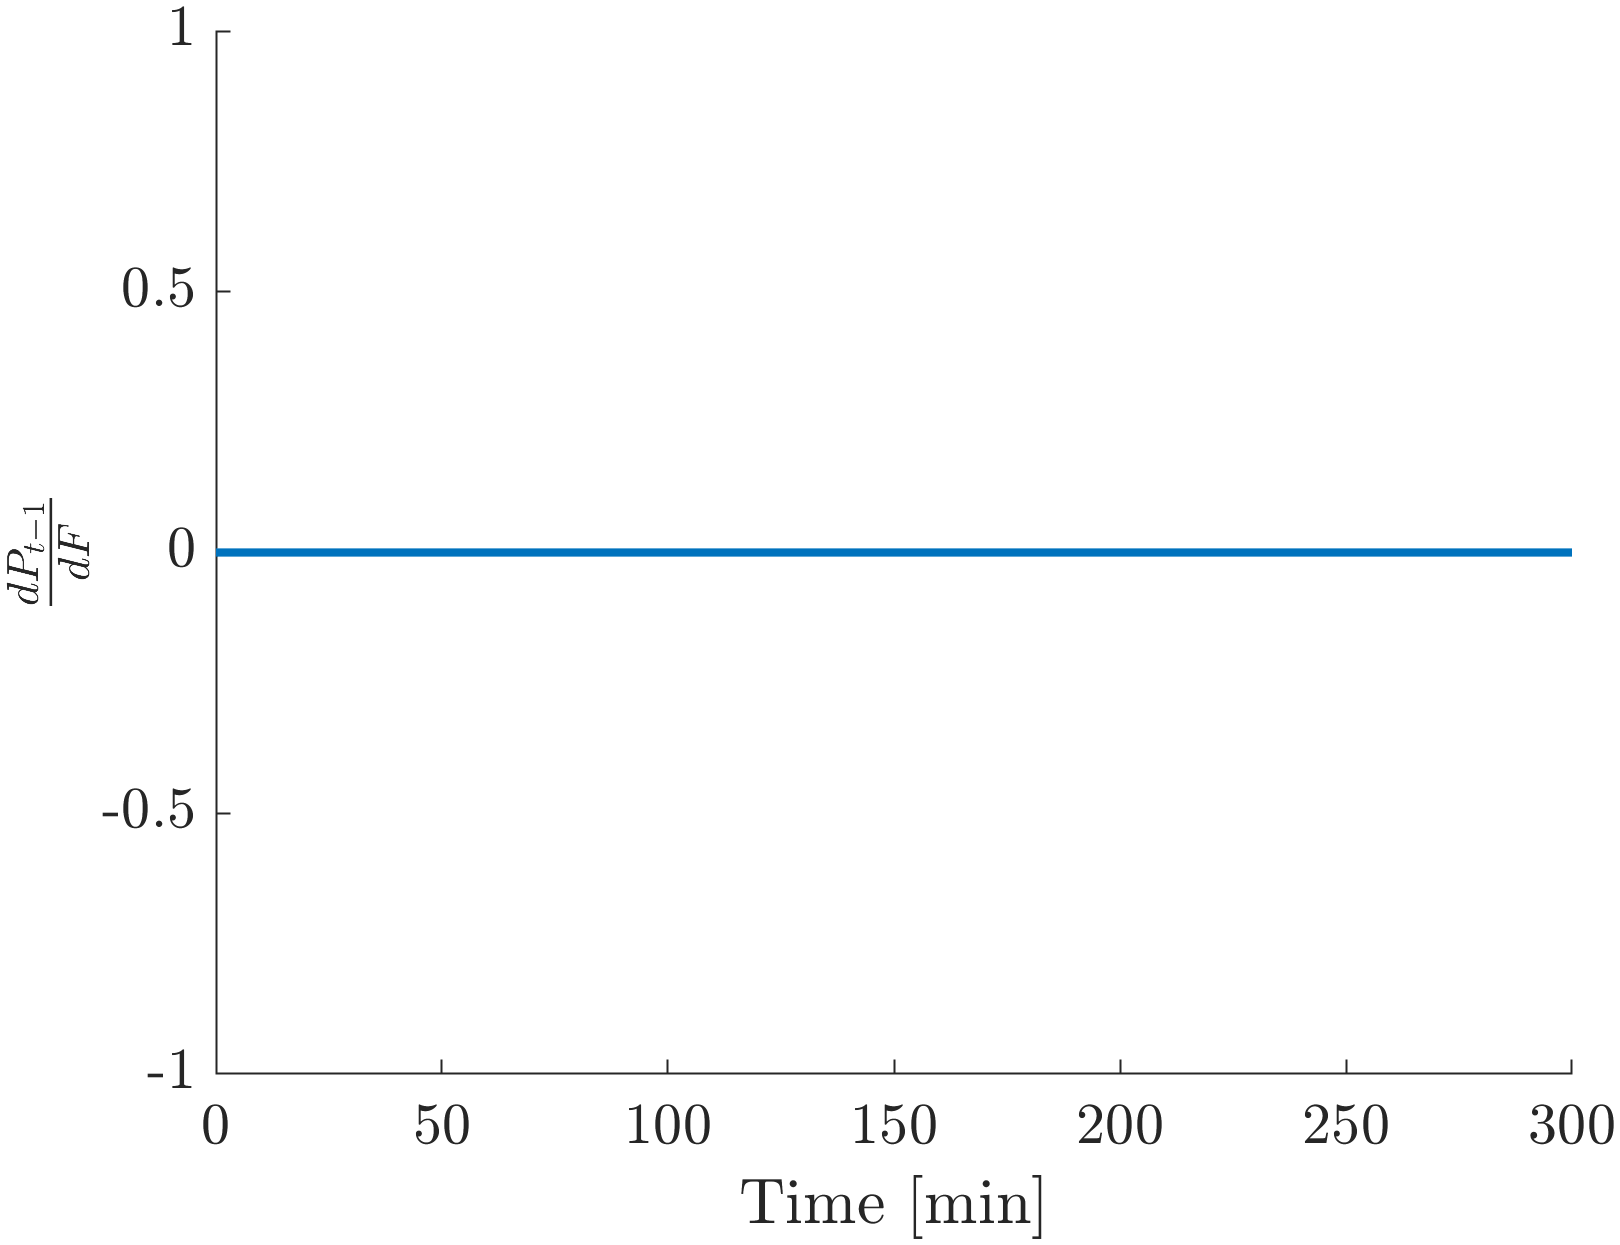
\includegraphics[trim = 0.0cm 0.0cm 0.0cm 0.0cm,clip,width=\columnwidth]{/Results_sensitivity/P_F.png}
		\caption{The effect of $F$ change on $P$}
		\label{fig:Sensitivty_F_P}
	\end{figure}
	
	It is important to note that $h$ represents enthalpy but not total enthalpy, thus excluding kinetic energy. As a consequence of the modelling assumptions, changes in $h$ and $\rho$ occur in response to changes in pressure or temperature, which explains no deviation of $h \times \rho$ in Figure \ref{fig:Sensitivty_F_H}.
    
    %When utilizing Dirichlet boundary conditions, it's crucial to be aware of potential numerical artefacts from the differing methods used to compute them. The system's enthalpy is determined through the time evolution of governing equations, while the inlet's enthalpy depends on the inlet temperature and pressure, which are the controls. A minor numerical mismatch between these values may manifest as an enthalpy difference propagating along the spatial domain. To ensure consistency between the fluid at the inlet and inside the computational domain, this analysis employs Neumann boundary conditions.
        
    \begin{figure}[h!]
    	\centering
    	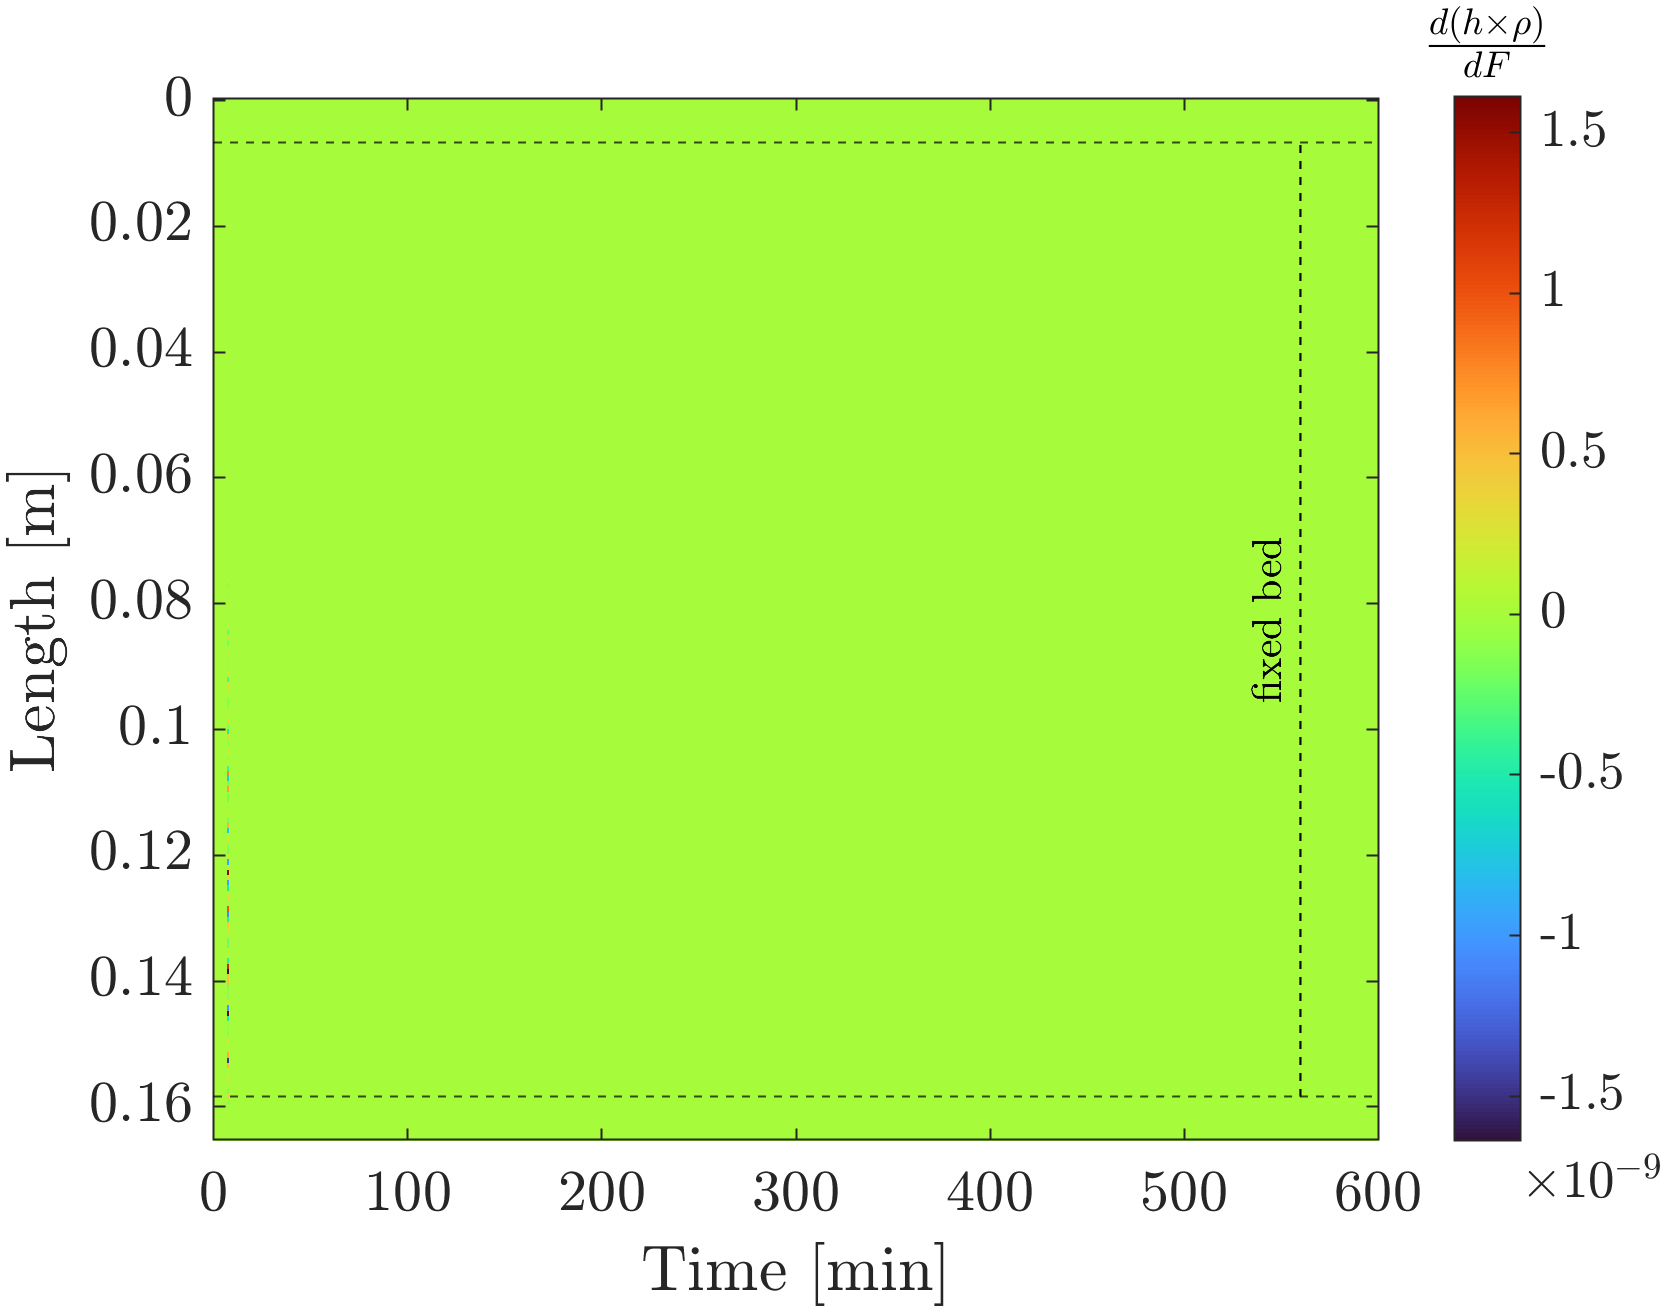
\includegraphics[trim = 0.0cm 0.0cm 0.0cm 0.0cm,clip,width=\columnwidth]{/Results_sensitivity/H_F.png}
    	\caption{The effect of $F$ change on $h \times \rho$}
    	\label{fig:Sensitivty_F_H}
    \end{figure}
   
   Figure \ref{fig:Sensitivty_F_CS} shows how the flow rate affects the solute concentration in the solid phase. At the beginning of the extraction process, the flow rate has a low impact on the extraction process due to the dominance of the concentration gradient in the kinetic regime. The corresponding sensitivities are close to zero. As time progresses, the increment in the mass flow rate has a greater influence on the extraction kinetics, causing the sensitivities to decrease towards their minimum values. Negative sensitivities indicate a faster extraction rate. Eventually, the amount of solute in the solid phase decreases, and the concentration gradient limits the extraction kinetic. This behaviour is represented by sensitivities, which increase from their minimal values and asymptotically approach to zero. In extreme cases, when all the solutes have been removed from the solid phase, the concentration gradient is zero, independent of the mass flow rate, which explains the asymptotic behaviour.
    
    \begin{figure}[h!]
    	\centering
    	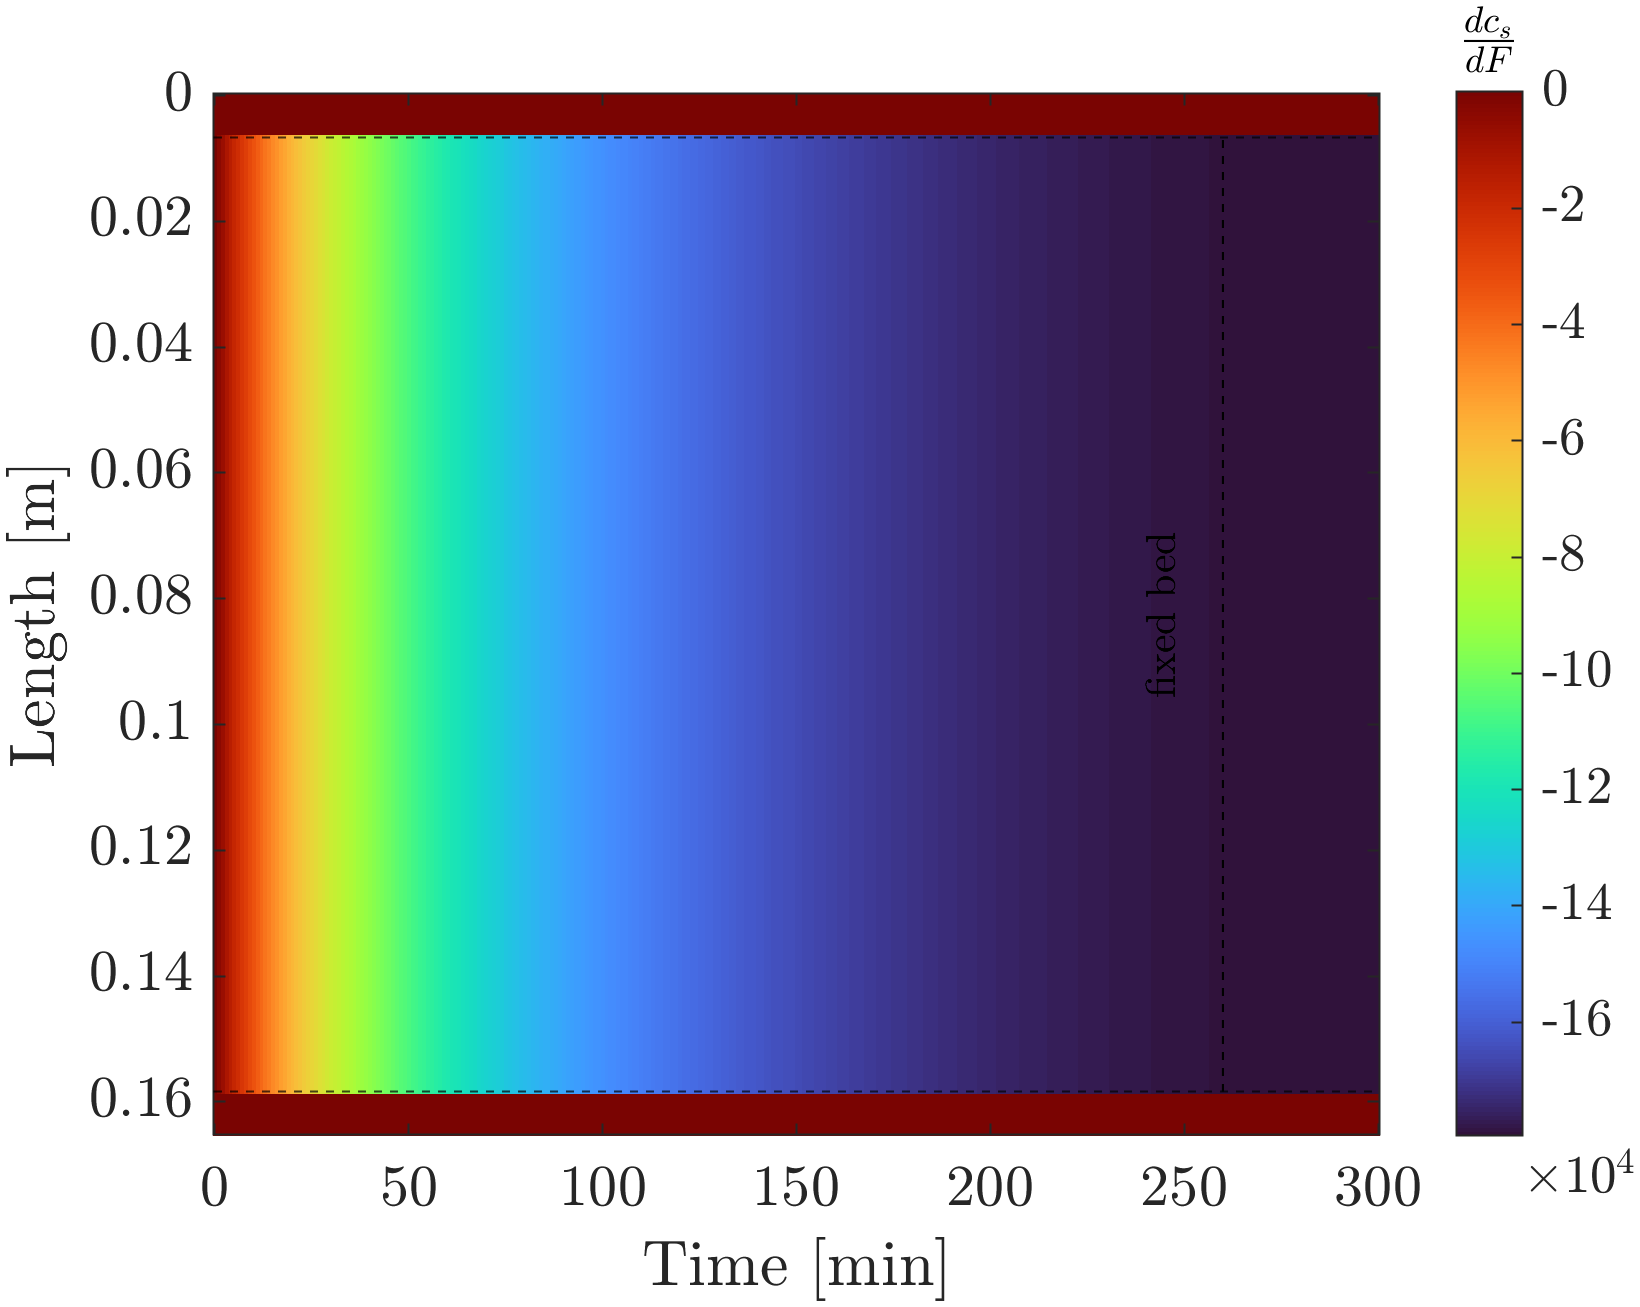
\includegraphics[trim = 0.0cm 0.0cm 0.0cm 0.0cm,clip,width=\columnwidth]{/Results_sensitivity/CS_F.png}
    	\caption{The effect of $F$ change on $C_s$}
    	\label{fig:Sensitivty_F_CS}
    \end{figure}
    
    Figure \ref{fig:Sensitivty_F_CF} illustrates how the concentration of solute in the fluid phase responds to an increase in the flow rate. Initially, sensitivities are close to zero, indicating a minimal system response. The growth in flow rate affects $C_f(z,t)$ indirectly by increasing the velocity and consequently elevating the concentration gradient. As a result, positive sensitivities emerge within the system, forming a front that progresses in the direction of flow. The positive front indicates that the larger amount of solute moves faster across the system. When the amount of the solute in the solid phase becomes a limiting factor, then the concentration gradient diminishes and slows down the extraction kinetics. The corresponding sensitivities form a front composed of negative sensitivities propagating through the extractor. The negative front indicates that the solute concentration in the fluid phase becomes lower than before the flow rate increment. Eventually, the negative sensitivities start to increase and asymptotically approach zero.
    
    \begin{figure}[h!]
    	\centering
    	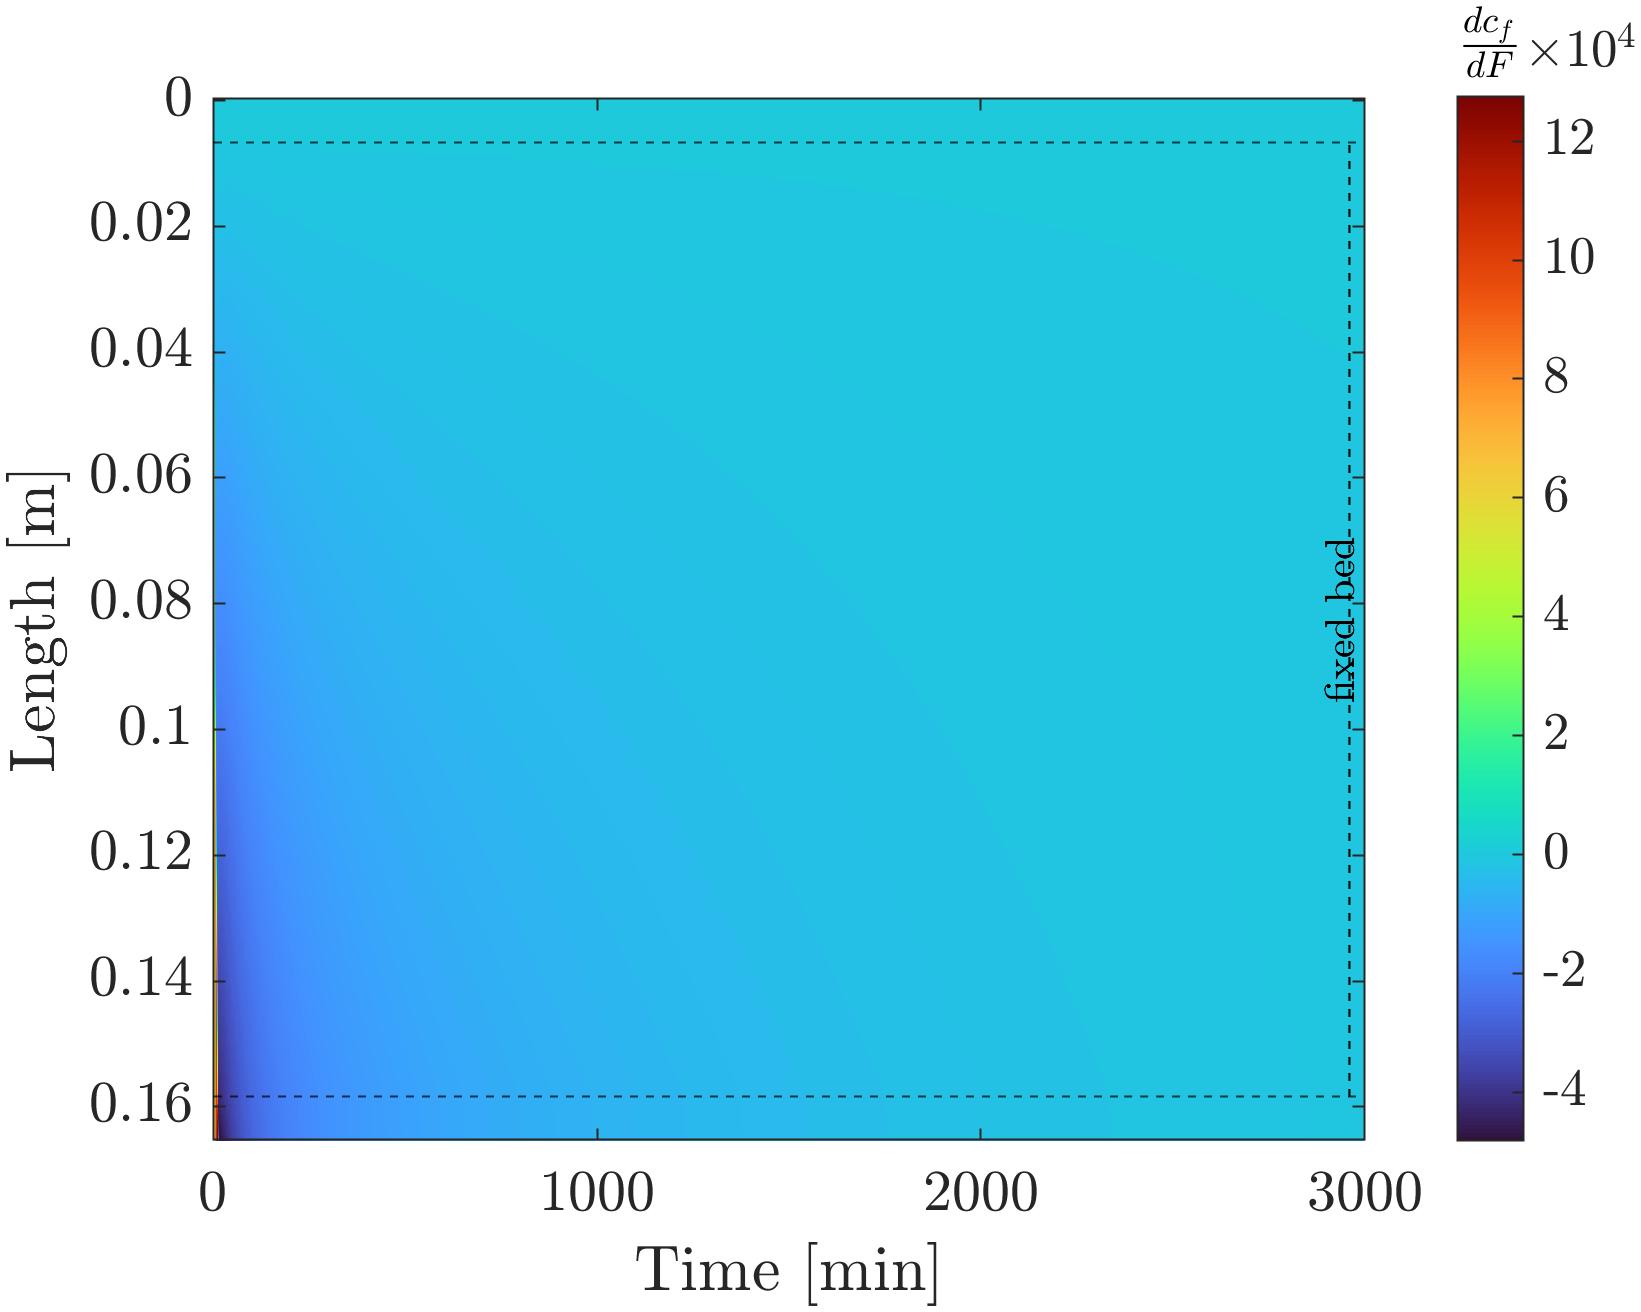
\includegraphics[trim = 0.0cm 0.0cm 0.0cm 0.0cm,clip,width=\columnwidth]{/Results_sensitivity/CF_F.png}
    	\caption{The effect of $F$ change on $C_f$}
    	\label{fig:Sensitivty_F_CF}
    \end{figure}

    Figure \ref{fig:Sensitivty_F_y} illustrates how the increase in flow rate affects the extraction yield. Initially, the sensitivity curve remains flat. This occurs because the fixed bed doesn't occupy the entire volume of the extractor. Hence, some time is required for the fluid to flow through the empty portion of the extractor to reach its outlet. Only when the solute in the fluid phase reaches the extractor's outlet can the yield be measured. After the idle time, the system response can be observed as the increment of  $dy/dF$. The positive sensitivity value indicates improved process efficiency, increasing yield. As time progresses, the sensitivity reaches its maximum and diminishes due to a decreasing concentration gradient. Eventually, $dy/dF$ asymptotically approaches zero. This happens because the amount of solute in the fluid phase becomes a limiting factor, and the process is in the diffusion regime.
    
    \begin{figure}[h!]
    	\centering
    	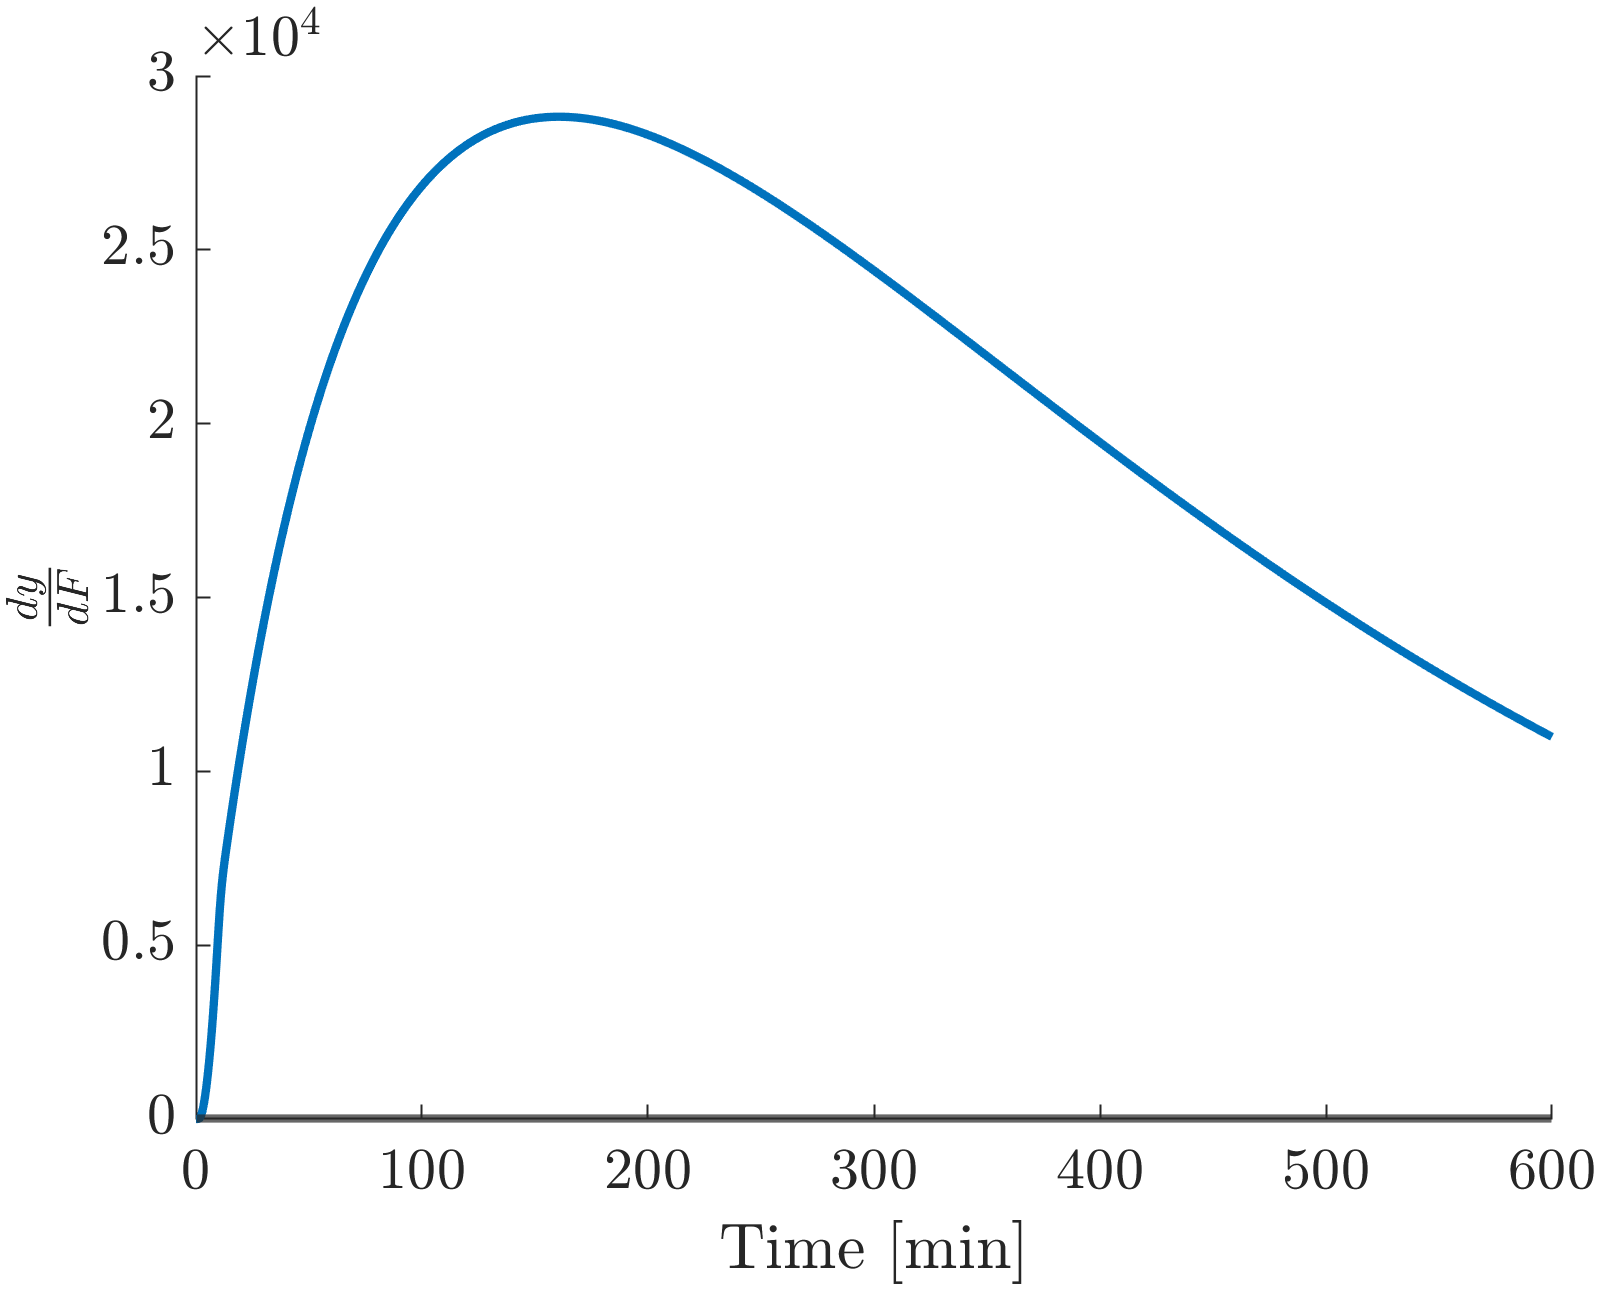
\includegraphics[trim = 0.0cm 0.0cm 0.0cm 0.0cm,clip,width=\columnwidth]{/Results_sensitivity/Y_F.png}
    	\caption{The effect of $F$ change on $y(t)$}
    	\label{fig:Sensitivty_F_y}
    \end{figure}
    
    \subsection{Pressure}
    
    As discussed in Chapter \ref{CH:Governing_equations_chapter}, a small pressure wave propagates at the speed of sound relative to the flow. If the flow velocity is relatively low, all pressure changes are hydrodynamic (resulting from velocity motion) rather than thermodynamic. The Low Mach-number assumption leads to instant propagation of the thermodynamic pressure throughout the system. This assumption allows considering a single pressure value for the entire system, as all changes occur simultaneously within the machine. Figure \ref{fig:Sensitivty_P_P} illustrates a step function representing the pressure change.
    
    \begin{figure}[h!]
    	\centering
    	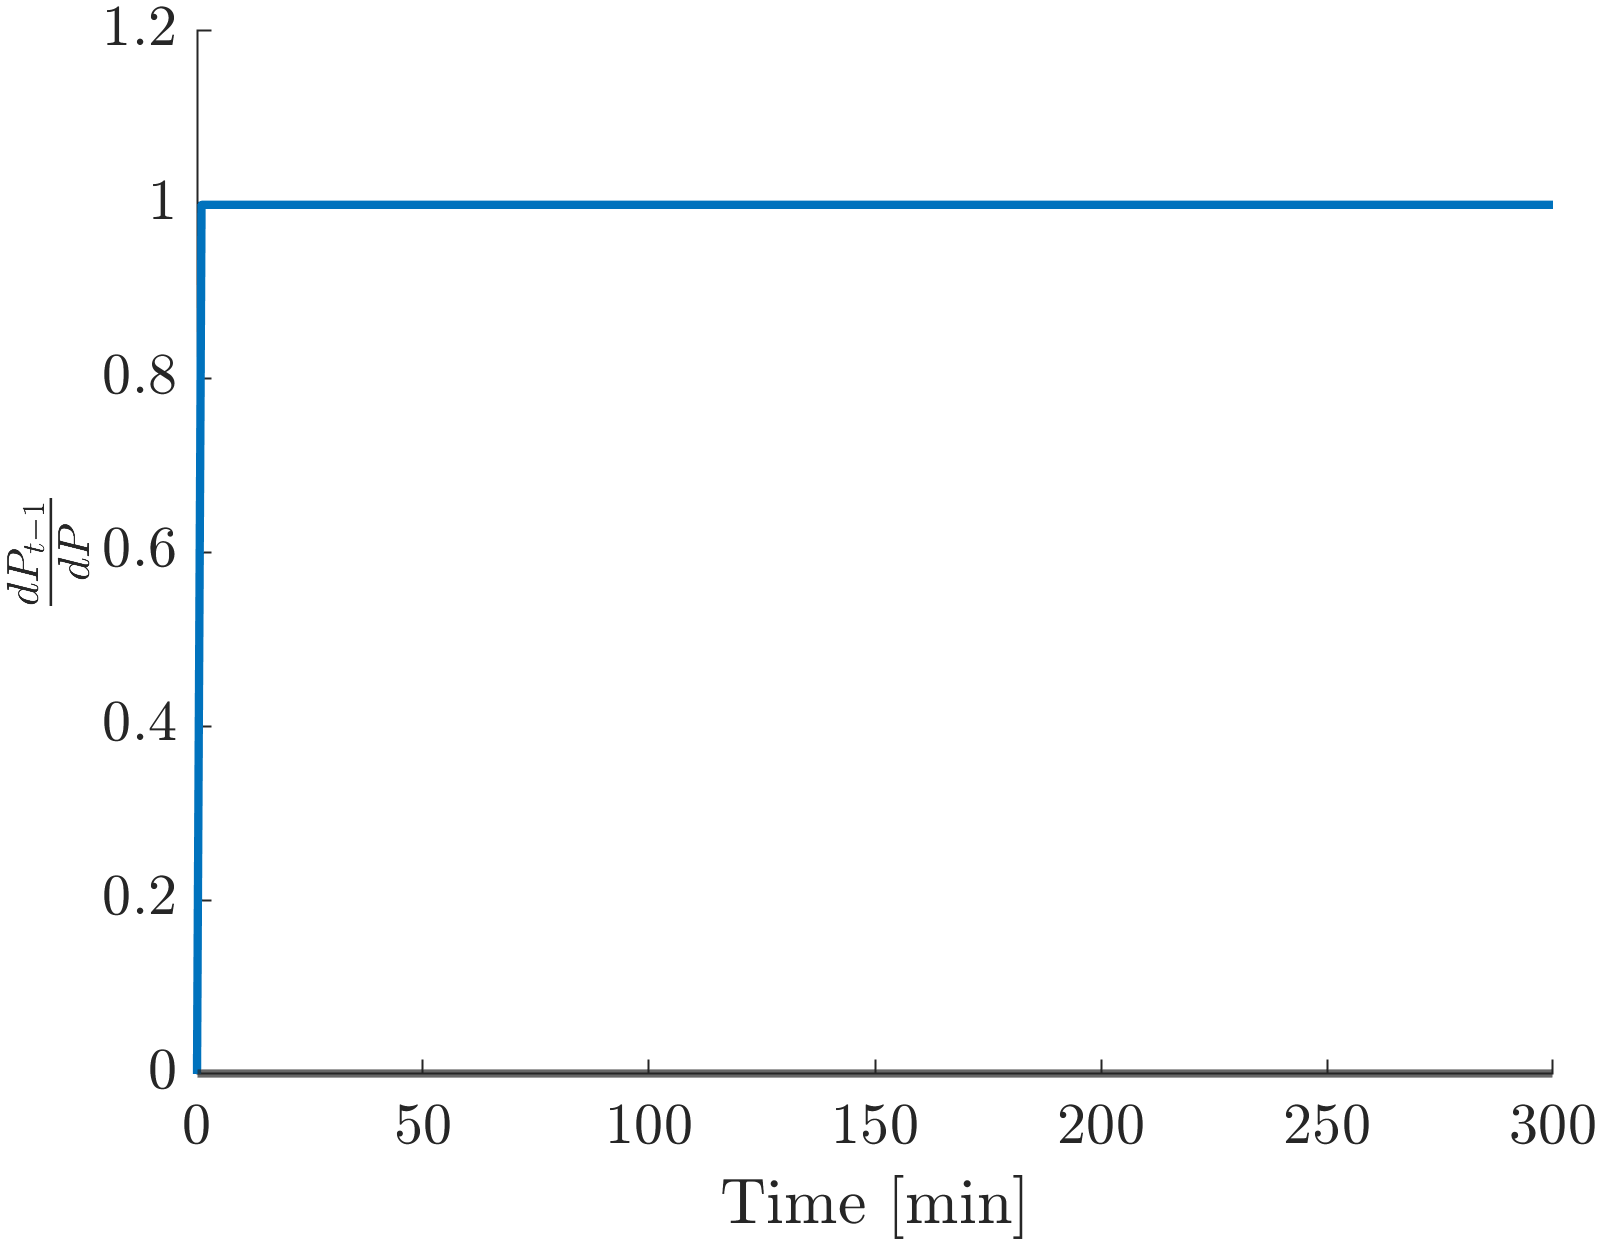
\includegraphics[trim = 0.0cm 0.0cm 0.0cm 0.0cm,clip,width=\columnwidth]{/Results_sensitivity/P_P.png}
    	\caption{The effect of $P$ change on $P$ in the system}
    	\label{fig:Sensitivty_P_P}
    \end{figure}
    
	According to Equation \ref{EQ:Enthalpy_equation}, the pressure change directly affects the quantity $h \times \rho$ through $\partial (P(t) A_f) / \partial t$, leading to the step change along the whole system, as presented in Figure \ref{fig:Sensitivty_P_H}. Depending on the configuration of the system, two cases are possible. If Dirichlet boundary conditions are applied, the inlet temperature is maintained at the predefined value and may differ from the temperature in the extractor. In such a case, the temperature difference will cause the heat front to propagate through the system. Alternatively, Neumann boundary conditions can be applied to ensure that the temperature inside the extractor matches that at its inlet. In this work, the second approach was chosen.
    
    \begin{figure}[h!]
    	\centering
    	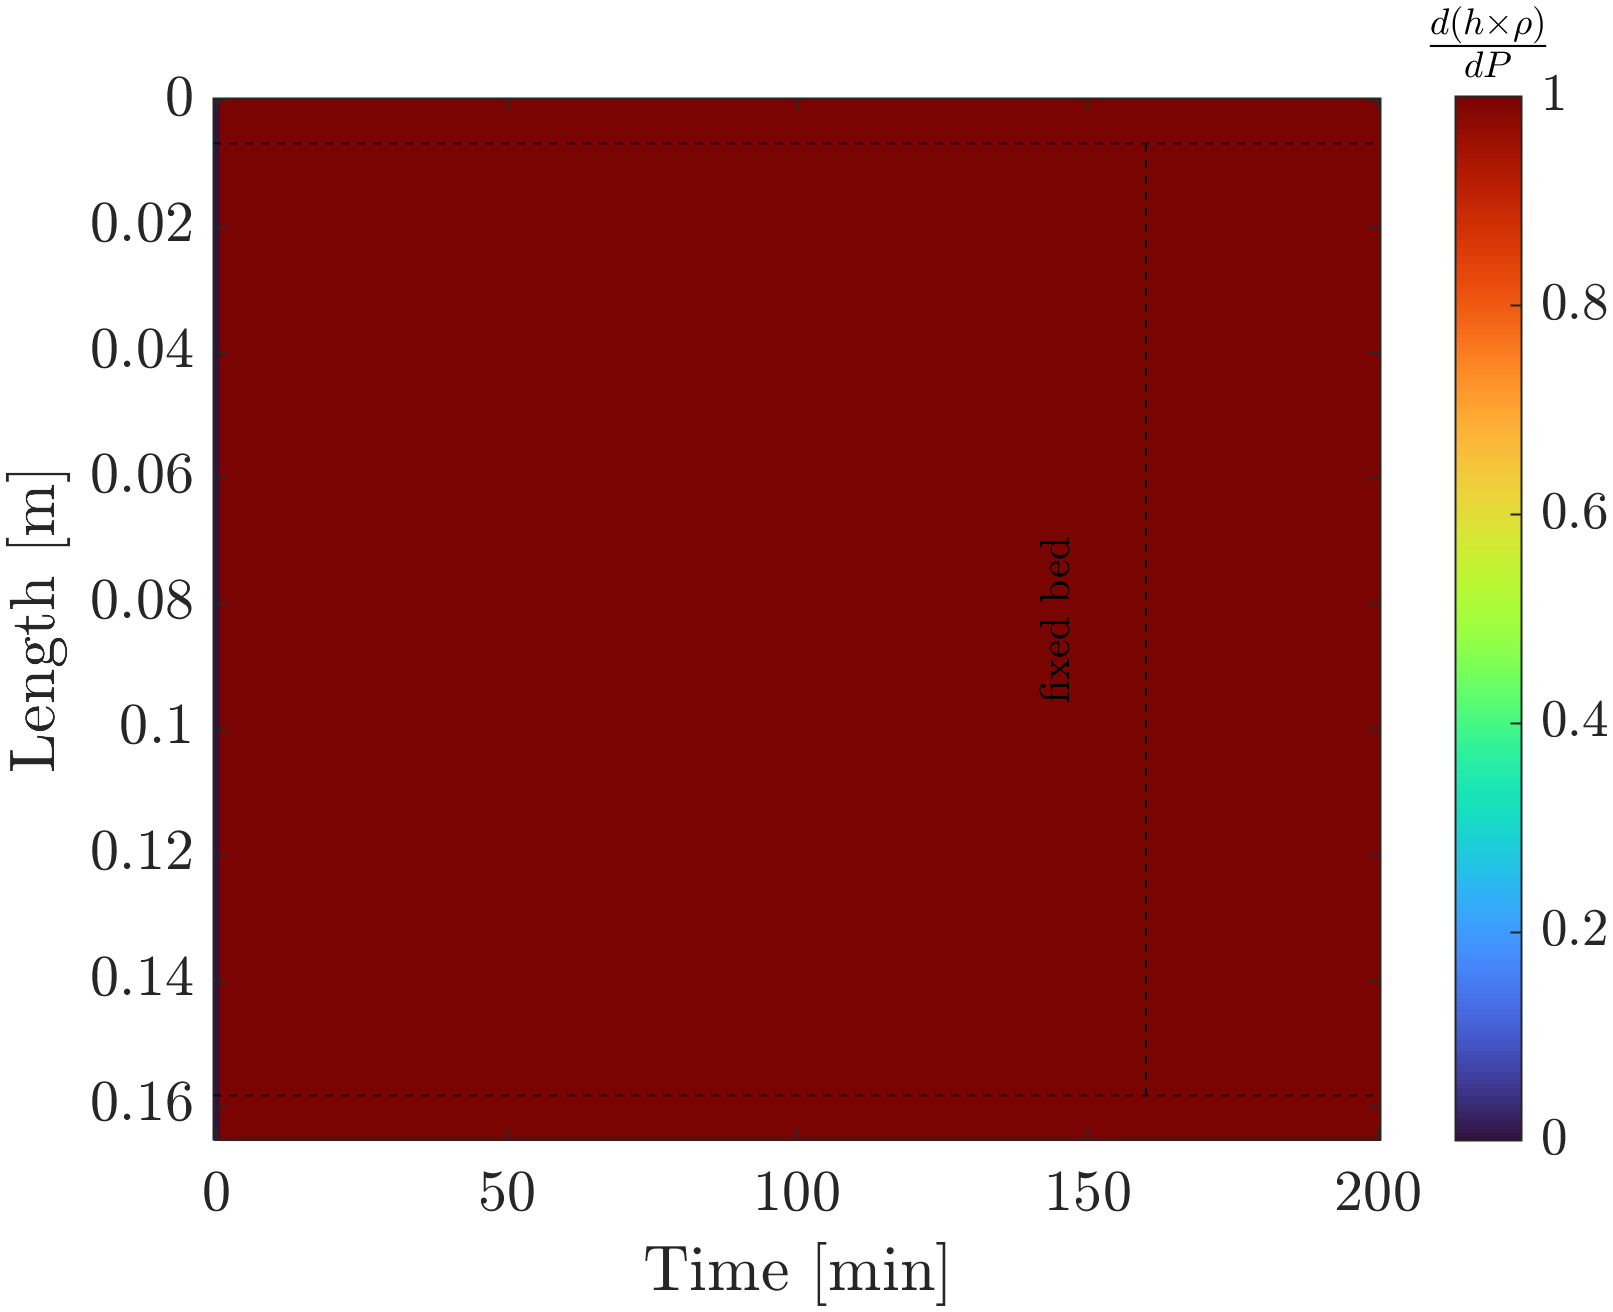
\includegraphics[trim = 0.0cm 0.0cm 0.0cm 0.0cm,clip,width=\columnwidth]{/Results_sensitivity/H_P.png}
    	\caption{The effect of $P$ change on $(h \times \rho)$ in the system}
    	\label{fig:Sensitivty_P_H}
    \end{figure}

	The pressure change affects the mass transfer in two ways. As discussed in Chapter \ref{CH: Continuity}, the velocity is inversely proportional to the density; hence, the higher density of the fluid leads to a lower velocity and larger residence time. The changes in the thermodynamic state of the fluid affect the extraction kinetic parameters, which are defined by correlations presented in {\color{red}article 1}. For example, the $D_i^R$ increases with the fluid density, which leads to a higher extraction rate. The cumulative effect of the pressure change on the solute concentration in the solid phase can be observed in Figure \ref{fig:Sensitivty_P_CS}. The sensitivity plot shows a close-to-uniform decay of sensitivities along the fixed bed. The negative values of sensitivities suggest a faster extraction rate. No matter the location of the sensitivity measure in the bed, the general behaviour stays the same. Every sensitivity starts with zero and decreases to a minimum value. After the extremum, the sensitivities asymptotically increase to zero.

	\begin{figure}[h!]
		\centering
		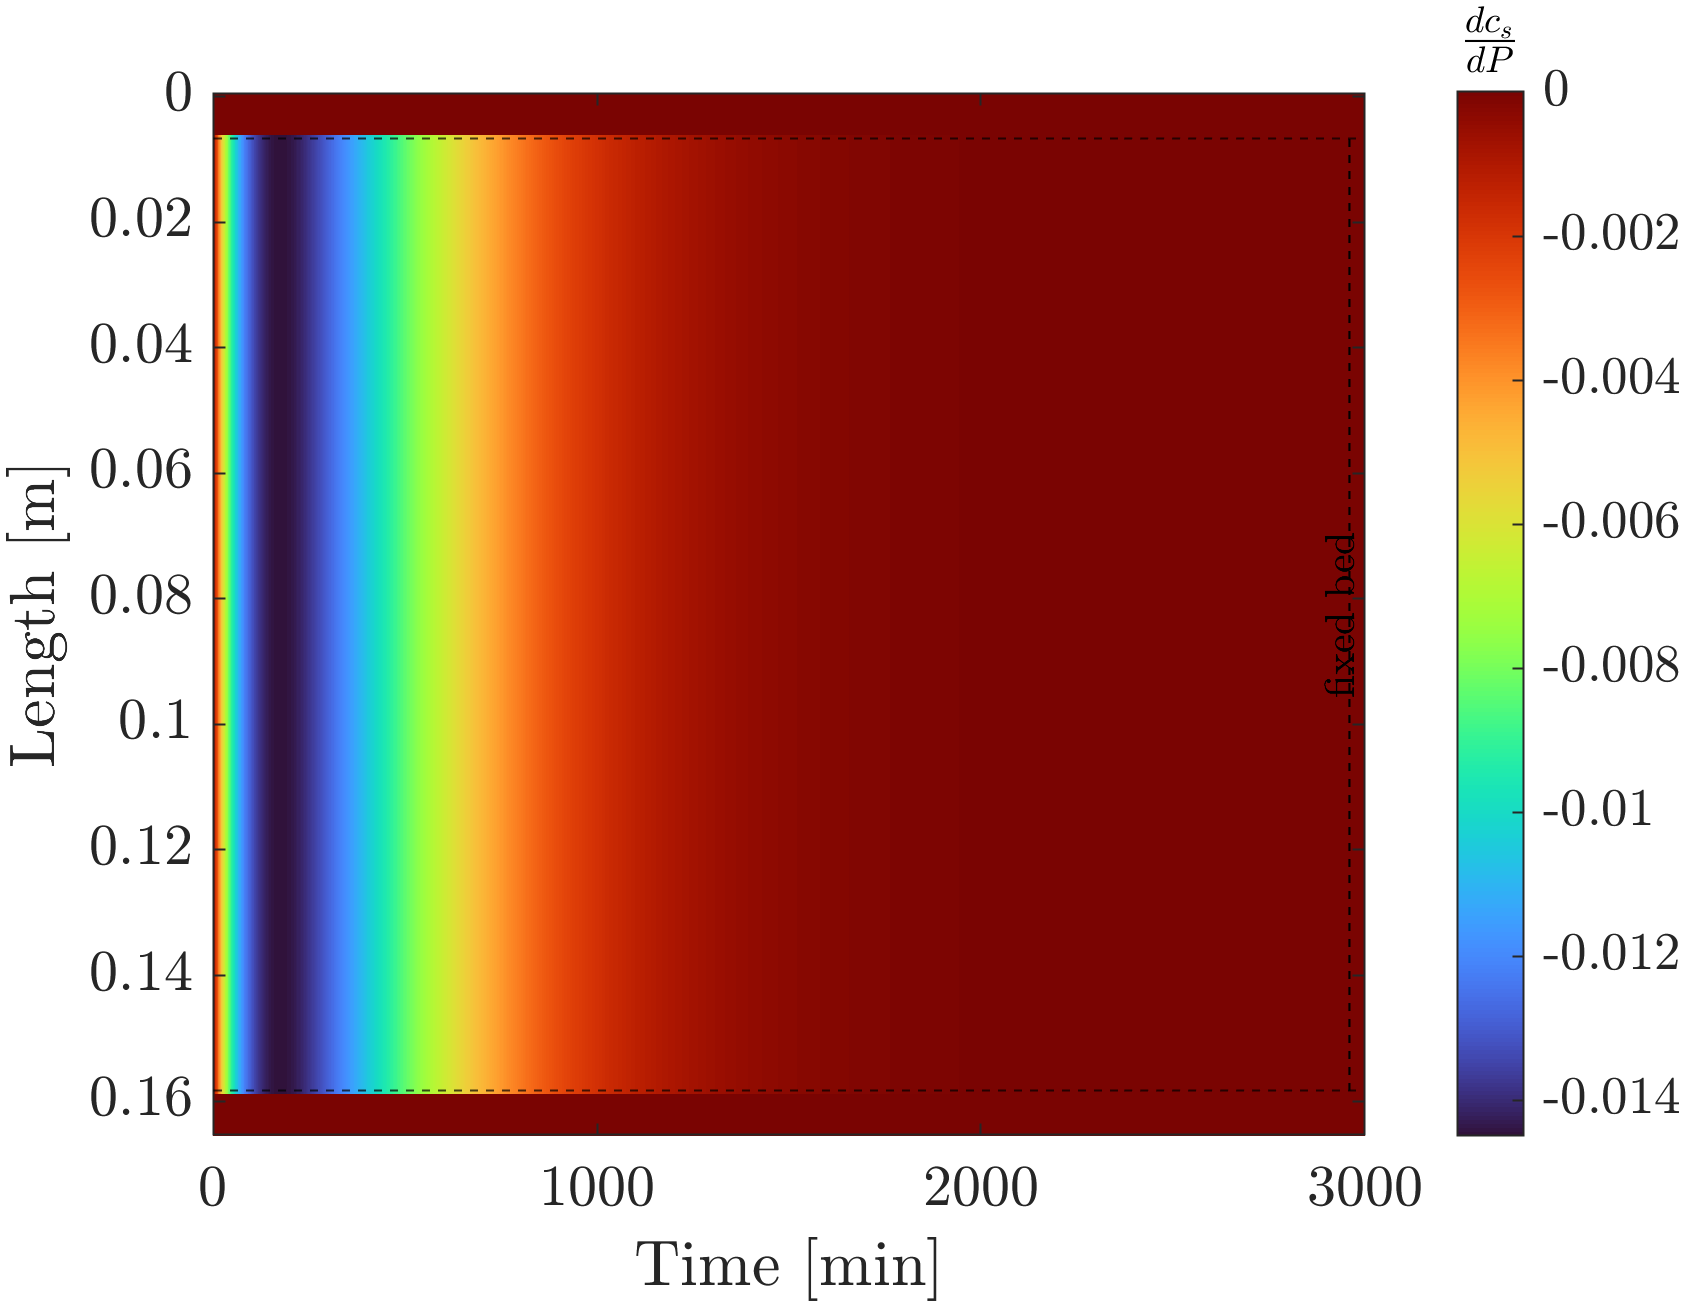
\includegraphics[trim = 0.0cm 0.0cm 0.0cm 0.0cm,clip,width=\columnwidth]{/Results_sensitivity/CS_P.png}
		\caption{The effect of $P$ change on $C_s$}
		\label{fig:Sensitivty_P_CS}
	\end{figure}

	The deviation in the solute concentration in the fluid phase caused by the pressure change is presented in Figure \ref{fig:Sensitivty_P_CF}. As discussed earlier, the sensitivities related to the solute concentration in the solid phase are characterized by negative sensitivities, suggesting a higher extraction rate due to the pressure change. Consequently, an increase in solute concentration in the fluid phase is expected. This increase in solute concentration in the fluid phase is visible in Figure \ref{fig:Sensitivty_P_CF} as positive sensitivities, which form a front that moves along the extractor. Due to the diffusion effect, the front changes its pattern in the empty section and becomes more spread. Accelerating the extraction rate since the beginning of the extraction process leads to a faster decrease in the concentration gradient. This effect is reflected in Figure \ref{fig:Sensitivty_P_CF} as the front of the negative sensitivities, which follows the positive front. Eventually, the negative sensitivities approach zero when the concentration gradient goes to zero.

	\begin{figure}[h!]
		\centering
		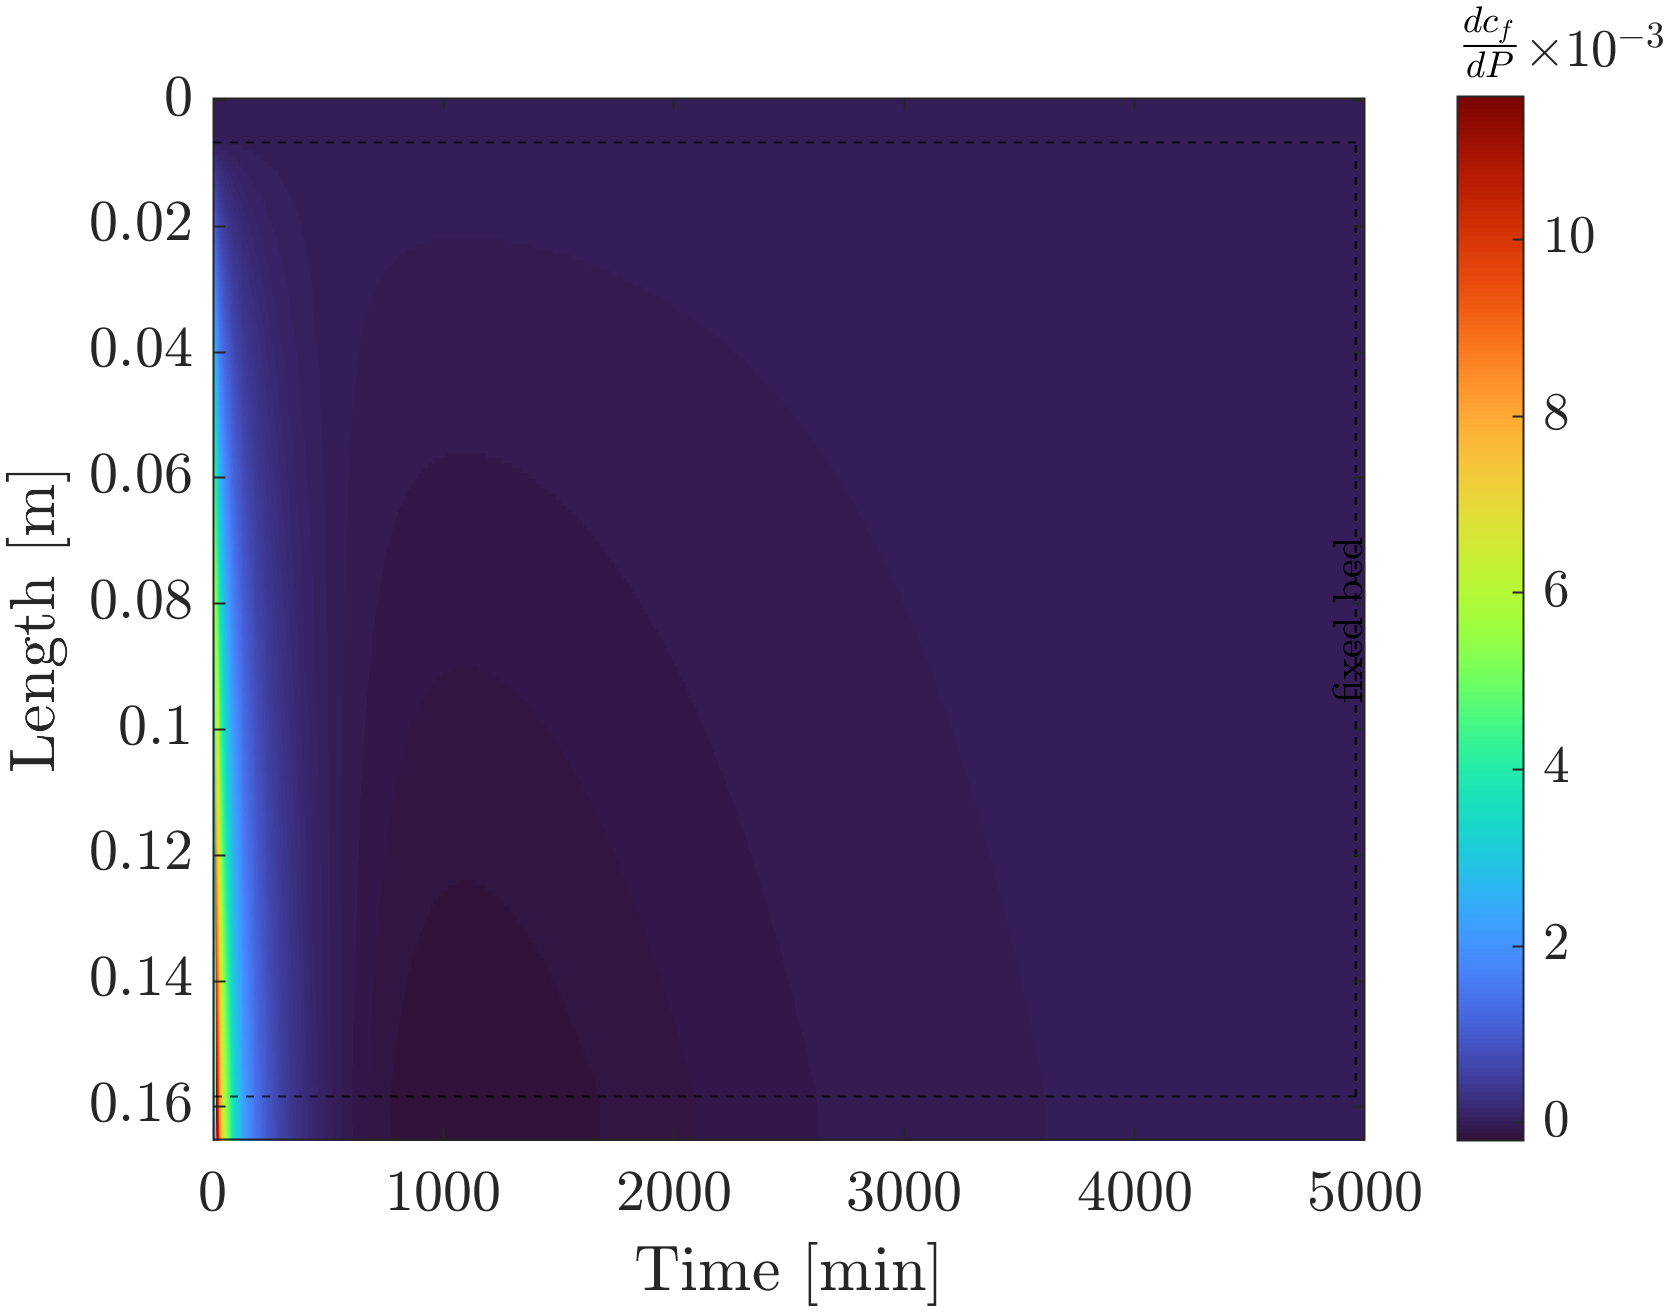
\includegraphics[trim = 0.0cm 0.0cm 0.0cm 0.0cm,clip,width=\columnwidth]{/Results_sensitivity/CF_P.png}
		\caption{The effect of $P$ change on $C_f$}
		\label{fig:Sensitivty_P_CF}
	\end{figure}

	The impact of pressure increase on extraction yield is depicted in Figure \ref{fig:Sensitivty_P_y}. The initial flat curve reflects a system delay caused by the empty space within the extractor that the fluid phase needs to flow through. The first observed deviation is a small negative sensitivity, which can be related to a lower fluid phase velocity. Keeping the same mass flow rate and increasing the density (by increasing the pressure) decreases the velocity. Next, the sensitivity rises, which indicates an increase in yield. $dy / dP$ reaches its positive maximum and then declines due to a limited amount of solute remaining in the solid phase. The sensitivity curve draws into negative values, reach a minimum point, and converges to zero. The simulation duration was extended to demonstrate the convergence of $dy / dP$ towards zero.

	\begin{figure}[h!]
		\centering
		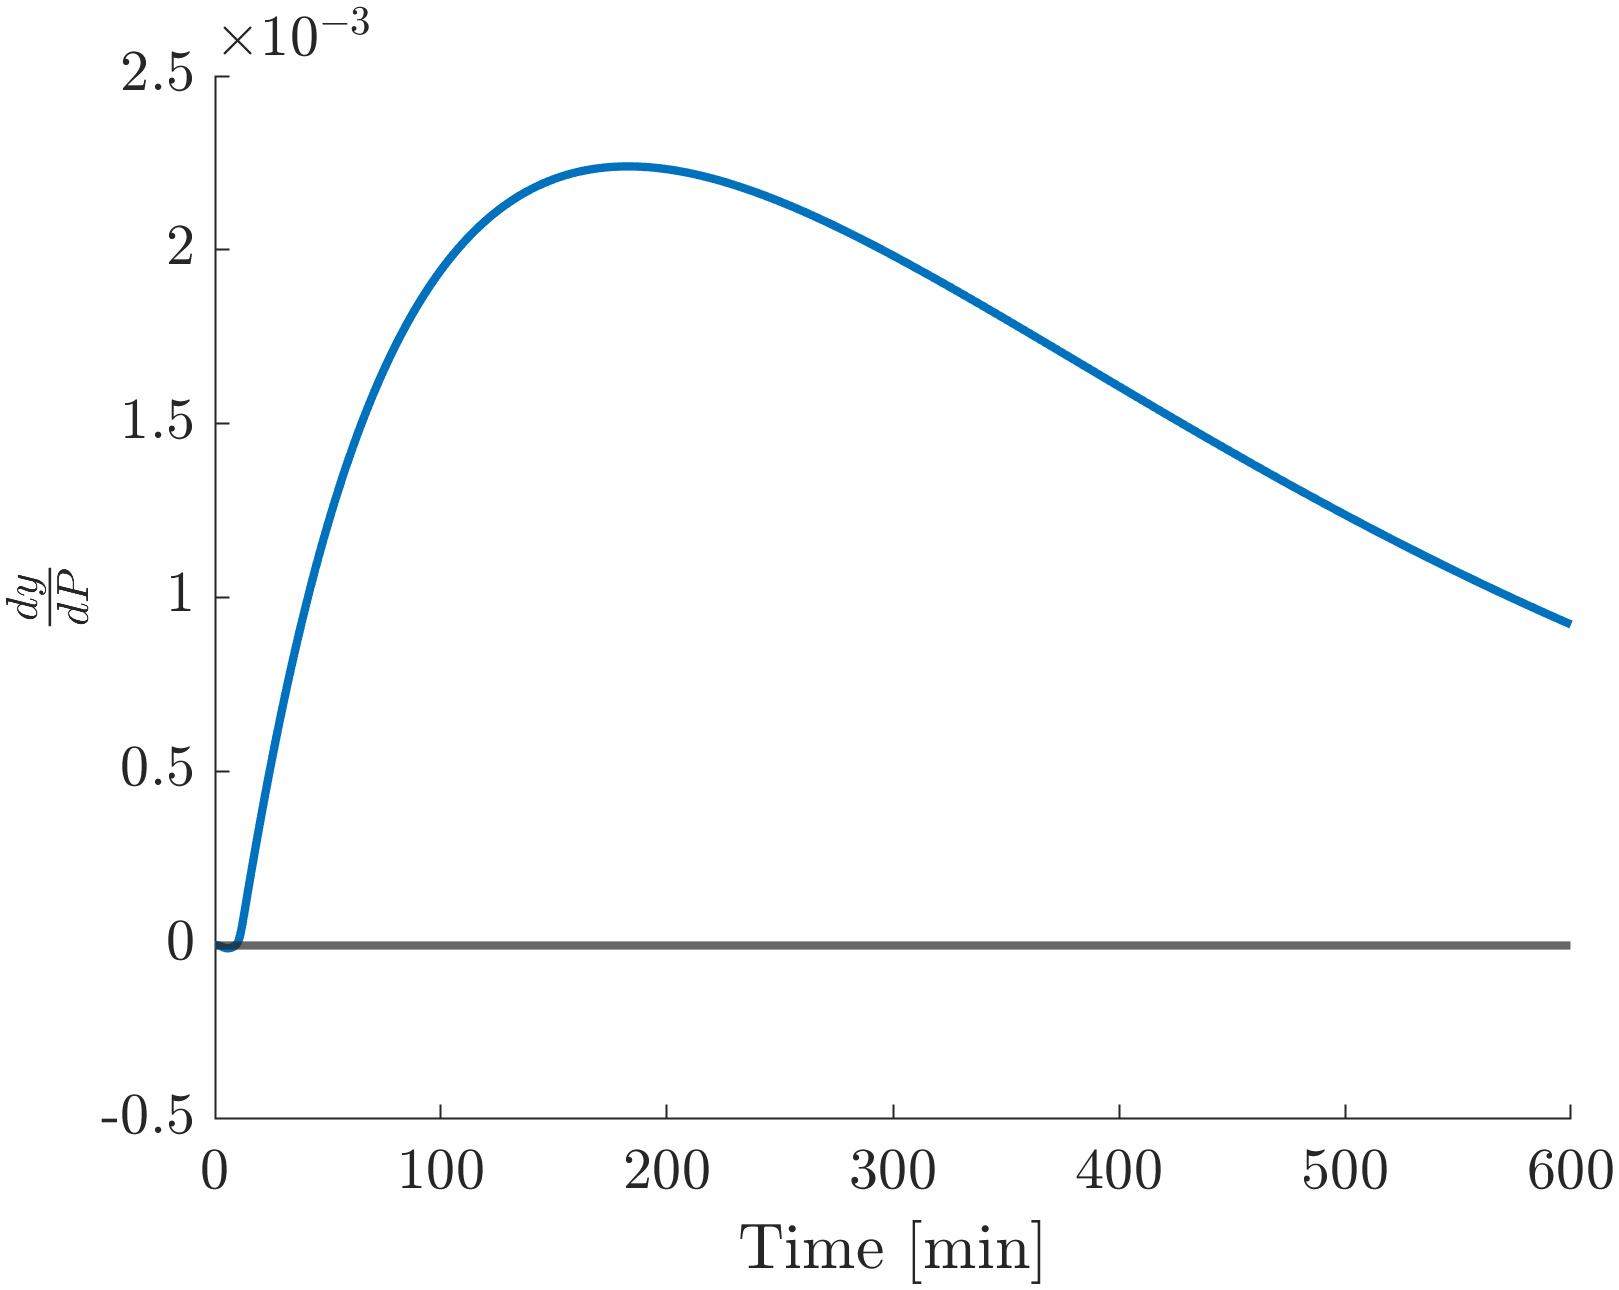
\includegraphics[trim = 0.0cm 0.0cm 0.0cm 0.0cm,clip,width=\columnwidth]{/Results_sensitivity/Y_P.png}
		\caption{The effect of $P$ change on $y(t)$}
		\label{fig:Sensitivty_P_y}
	\end{figure}

	\subsection{Inlet temperature}
	
	The sensitivity analysis of the inlet temperature differs from the two cases presented earlier because the perturbation does not affect the entire system instantaneously; instead, it propagates through the system.
	
	The Figure \ref{fig:Sensitivty_P_T} for the system pressure response shows a flat curve, indicating an invariant behavior of pressure in response to inlet temperature changes throughout the time. This uniformity is expected, as explained in the Chapter XXX. The pressure of the modelled system is controlled and maintained independently of the inlet temperature variations. 
	%The sensitivity analysis of the inlet temperature differs from the two cases presented earlier because the perturbation does not affect the entire system instantaneously; instead, it propagates through the system. As the fluid with the modified temperature flows along the system, it gradually modifies the mass transfer parameters. One important assumption is that the inlet temperature change does not affect the pressure, which explains a horizontal line in Figure \ref{fig:Sensitivty_P_T}.
	
	\begin{figure}[h!]
		\centering
		\includegraphics[trim = 0.0cm 0.0cm 0.0cm 0.0cm,clip,width=\columnwidth]{/Results_sensitivity/P_T_{in}.png}
		\caption{The effect of $T_{in}$ change on $P$ in the system}
		\label{fig:Sensitivty_P_T}
	\end{figure}

	The inlet temperature is characterized by the Dirichlet boundary condition. The boundary value of $(h\times \rho)$ is calculated based on two controls which can be manipulated: inlet temperature and given pressure. Any deviation in $T_{in}$ affects $(h\times \rho)$ at the inlet, propagating according to the governing equations.
	Figure \ref{fig:Sensitivty_T_H} showcases the sensitivity of the fluid enthalpy to the inlet temperature over both time and the length of the extraction bed. The heat front propagation from the inlet of the extractor to its outlet. The fluid entering the extraction bed will have its enthalpy most influenced by the inlet conditions. As the fluid progresses through the bed, the enthalpy change sensitivity affects the whole system gradually. Over time, the system's gradual approach to a new thermal steady state and the sensitivities becomes zero.
	
	%The heat front propagation is presented in Figure \ref{fig:Sensitivty_T_H}. The initial system had constant temperature along the whole spatial domain. 
	
	\begin{figure}[h!]
		\centering
		\includegraphics[trim = 0.0cm 0.0cm 0.0cm 0.0cm,clip,width=\columnwidth]{/Results_sensitivity/H_T_{in}.png}
		\caption{The effect of $T_{in}$ change on $(h \times \rho)$ in the system}
		\label{fig:Sensitivty_T_H}
	\end{figure}

	Figure \ref{fig:Sensitivty_T_CS} shows the curve depicts an initial sharp increase (positive sign of the sensitivities) in the solute concentration in the solid phase as a function of time, which then asymptotically approaches a stable value before increasing again towards the end of the period. Although $D_i^R$ decrease with the fluid's density, the $\Upsilon$ increases, which explains the system responses. This suggests that an increase in inlet temperature initially slow down the mass transfer of solutes from the solid phase to the supercritical fluid, hence the concentration of the solute in the solid phase increases. Over time, this effect stabilizes, which could indicate the exhaustion of easily extractable solutes.
	%Figure \ref{fig:Sensitivty_T_CS} illustrates how the change in inlet temperature affects the concentration of solute in the solid phase. As presented in {\color{red}article 1}, the value of $D_i^R$ decreases as density decreases. Therefore, it is expected to observe positive sensitivities in Figure \ref{fig:Sensitivty_T_CS}, indicating a slower extraction rate. Initially, the sensitivities are zero along the fixed bed because the heat front requires time to reach the fixed bed. Since this propagation is not instantaneous, a non-uniform distribution of sensitivities along the fixed bed becomes evident. All the sensitivities gradually increase until they reach their maximum. When the concentration gradient becomes the limiting factor, the sensitivities decrease.

	\begin{figure}[h!]
		\centering
		\includegraphics[trim = 0.0cm 0.0cm 0.0cm 0.0cm,clip,width=\columnwidth]{/Results_sensitivity/CS_T_{in}.png}
		\caption{The effect of $T_{in}$ change on $C_s$ in the system}
		\label{fig:Sensitivty_T_CS}
	\end{figure}

	The Figure \ref{fig:Sensitivty_T_CF} represents the sensitivity of the concentration of solutes in the fluid phase over a period of 600 minutes as a result of changes in the inlet temperature. Initially, all the sensitivities remain at zero due to the idle period. As the fluid with elevated temperature flows through the fixed bed, the internal mass transfer slows down (the $D_i^R$ is proportional to density as presented in {\color{red}article 1}), resulting in negative sensitivities. The negative sensitivities can be explained by considering that the heat front slowed mass transfer, causing more solute to remain in the solid phase. After reaching their minima, the sensitivities increase and reach positive values. Later the sensitivities starts to increase due higher concentration gradient if compared to before the temperature change. Eventually, the system response stabilize around a constant value when the extraction kinetics become a limiting factor.
	
	\begin{figure}[h!]
		\centering
		\includegraphics[trim = 0.0cm 0.0cm 0.0cm 0.0cm,clip,width=\columnwidth]{/Results_sensitivity/CF_T_{in}.png}
		\caption{The effect of $T_{in}$ change on $C_f$ in the system}
		\label{fig:Sensitivty_T_CF}
	\end{figure}

	Figure \ref{fig:Sensitivty_T_y} depicts how an increase in inlet temperature alters the extraction yield. Initially, the sensitivity curve remains flat due to the idle time. The first observed response of the system is a small increment of the $dy/dT_{in}$ caused by an increment of the velocity( which is inversely proportional to the fluid density). After the small positive peak, the sensitivity curve begins to decrease. The negative value of the sensitivity indicates a lower process efficiency. Over time, the sensitivity reaches its minimum and then increases due to a higher concentration gradient than in the case without the disturbance. Eventually, the $dy/dT_{in}$ curve flattens around a negative value. The flattening of the yield curve suggests that the mass transfer parameters limit the extraction rate, and the residual solute in the solid phase becomes difficult to obtain. The simulation time was extended to show how the sensitivity plot flattened.

	\begin{figure}[h!]
		\centering
		\includegraphics[trim = 0.0cm 0.0cm 0.0cm 0.0cm,clip,width=\columnwidth]{/Results_sensitivity/Y_T_{in}.png}
		\caption{The effect of $T_{in}$ change on $y(t)$ in the system}
		\label{fig:Sensitivty_T_y}
	\end{figure}
	
\end{document}


































